\chapter{INTRODUCTION}
\label{chap:intro}

The installed capacity of solar power in the US continues to grow as a
result of aging coal and natural gas power plants, lower costs,
state renewable portfolio standards, and efforts to decarbonize the
electrical grid.
As shown in \Cref{fig:solarinstall}, this growth has been steady since 2010 and shows no signs of abating.

\begin{figure}[ht]
  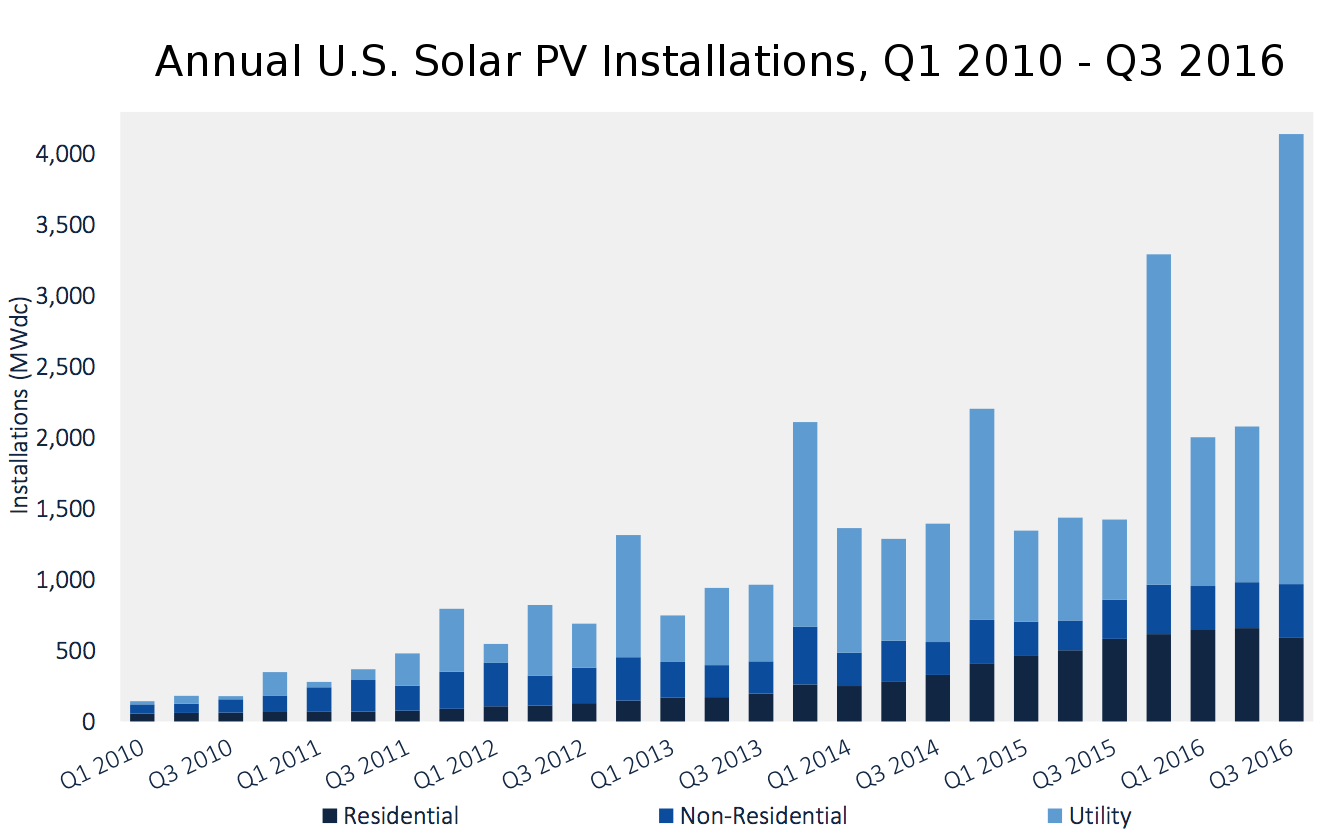
\includegraphics[width=\textwidth]{figs/solar_installations.png}
  \caption[Annual installations of solar PV in the US]{Annual
    installations of solar photovoltaic (PV) systems in the
    US. [Source:~\cite{GTM/SEIA2016}]}
\label{fig:solarinstall}
\end{figure}

Solar irradiance is the fuel that drives all solar power plants.
Unlike sources of fuel for conventional power generators like coal or
natural gas, the solar resource is highly variable due to the nature
of the chaotic system that is weather.
This variability of the solar resource leads to uncertainty at the
electric utility and increases management costs \citep{Joskow2011}.
Forecasts help utilities manage the variability in a number of ways
\citep{Kleissl2013,Inman2013}, including the optimal dispatch of
battery storage \citep{Cormode2015}.

This dissertation will explore solar irradiance forecasting at short
time horizons (now to two hours in the future) made possible by an
irradiance monitoring network.
First, the current state of solar power in the Southwest US and a
brief overview of forecasting methods will be discussed.

\section{State of Solar Power in the Southwest}

\section{Solar Irradiance Forecasting}
resource assessment
short term
wrf
climatology

\section{This Dissertation in Brief}

\begin{figure}[h]
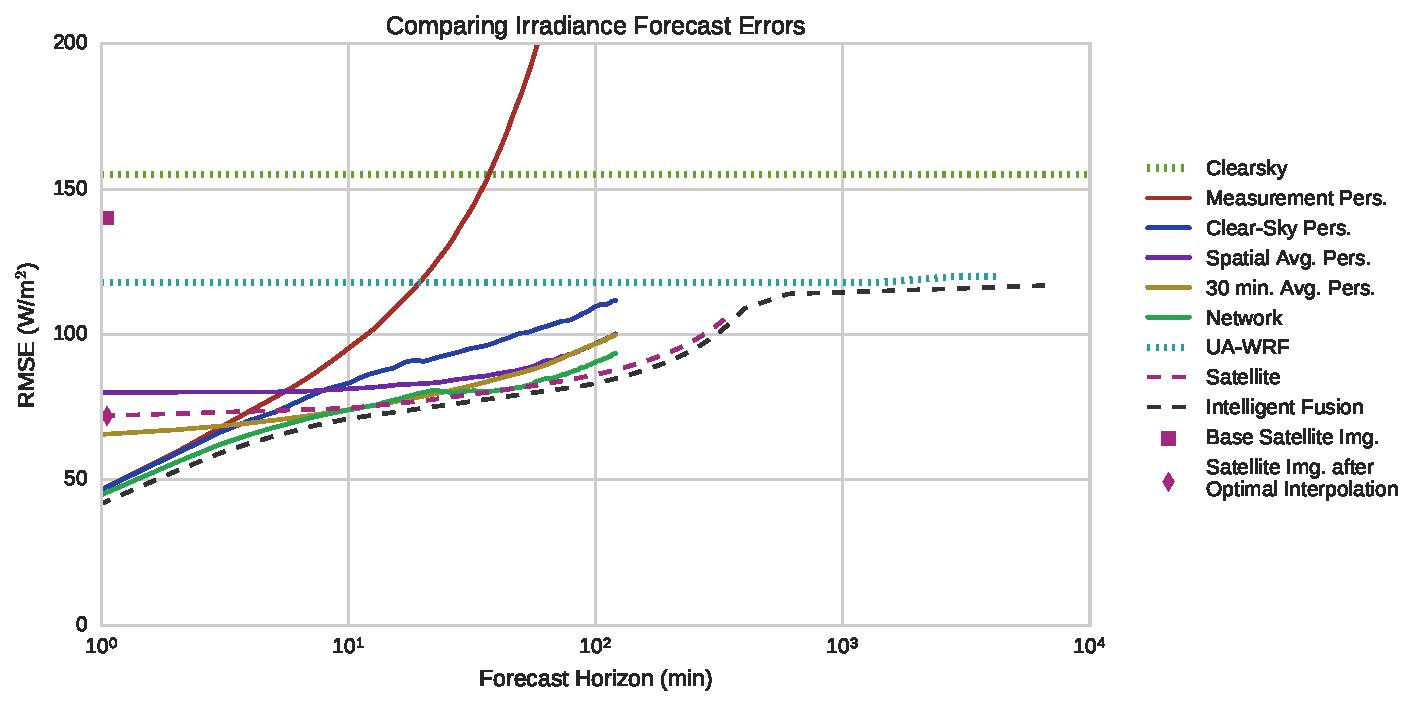
\includegraphics[width=\textwidth]{figs/timehorizon.pdf}
\caption[Irradiance forecast errors across forecast horizons]{A
  comparison of irradiance forecast root-mean squared errors (RMSE)
  across many time horizons. The solid lines (and points) indicate
  forecasts that will be studied in depth in this dissertation. Dashed
  lines are based on prelimnary analysis, but have not been studied in
  depth. Pers.\ refers to persistence, and UA-WRF refers to the
  numerical weather models generated at the UA using the Weather
  Research and Forecasting (WRF) model. The optimal grinding is a
  theoretical combination of forecasts at diffferent time horizons for
  the best forecast at all horizons. The persistence and network
  forecasts will be discussed in \Cref{chap:network} and the satellite
  image points will be discussed in \Cref{chap:satoi}.}
\label{fig:bullshitplot}
\end{figure}




%%% Local Variables:
%%% mode: latex
%%% TeX-master: "dissertation"
%%% End:
